% Exercise Template
%A LaTeX template for typesetting exercise in Persian (with cover page).
%By: Reza Adinepour

\documentclass[12pt]{exam}

\usepackage{setspace}
\usepackage{listings}
\usepackage{graphicx,subfigure,wrapfig}
\usepackage{multirow}
\usepackage{matlab-prettifier}
\usepackage{amsmath}
\usepackage{xcolor}
\usepackage{multicol}
\usepackage[T1]{fontenc}
\usepackage{beramono}% monospaced font with bold variant


\usepackage[margin=20mm]{geometry}
\usepackage{xepersian}
\settextfont{XB Niloofar}

\newcommand{\class}{آزمایشگاه FPGA}
\newcommand{\term}{نیم‌سال دوم ۰۱-۰۲}
\newcommand{\college}{دانشکده مهندسی برق}
\newcommand{\prof}{استاد: دکتر خرقانیان}

\singlespacing
\parindent 0ex

\begin{document}


% -------------------------------------------------------
%  Thesis Information
% -------------------------------------------------------

\newcommand{\ThesisType}
{سمینار}  % پایان‌نامه / رساله
\newcommand{\ThesisDegree}
{کارشناسی ارشد گرایش معماری کامپیوتر}  % کارشناسی / کارشناسی ارشد / دکتری
\newcommand{\ThesisMajor}
{مهندسی برق}  % مهندسی کامپیوتر
\newcommand{\ThesisTitle}
{موضوع آزمایش}
\newcommand{\ThesisAuthor}
{رضا آدینه پور-9814303\\علی‌رضا قربانی-9823263}
\newcommand{\ThesisSupervisor}
{جناب آقای دکتر رضا خرقانیان}
\newcommand{\ThesisDate}
{اردی‌بهشت 1402}
\newcommand{\ThesisDepartment}
{دانشکده مهندسی برق}
\newcommand{\ThesisUniversity}
{دانشگاه صنعتی شاهرود}

% -------------------------------------------------------
%  English Information
% -------------------------------------------------------

\newcommand{\EnglishThesisTitle}{A Standard Template for Course Exercise}


\pagestyle{empty}

\begin{center}


\includegraphics[scale=0.17]{images/logo.png}

\vspace{0.5cm}
\ThesisUniversity \\[-0.3em]
\vspace{0.5cm}
\ThesisDepartment\\

\begin{large}
\vspace{0.5cm}


%\ThesisMajor

\end{large}

\vspace{1.5cm}

{عنوان:}\\[1.2em]
{\LARGE\textbf{\ThesisTitle}}\\ 
\vspace{1cm}
% \begin{latin}
% {\Large\textbf\EnglishThesisTitle}
% \end{latin}

\vspace{2cm}

{نگارش}\\[.5em]
{\large\textbf{\ThesisAuthor}}

\vspace{1.5cm}

{استاد مربوطه}\\[.5em]
{\large\textbf{\ThesisSupervisor}}

\vspace{1cm}



\vspace{2cm}

\ThesisDate

\end{center}

\newpage


% These commands set up the running header on the top of the exam pages
\pagestyle{head}
\firstpageheader{}{}{}
\runningheader{صفحه \thepage\ از \numpages}{}{\class}
\runningheadrule

\vspace{0pt}

\lstdefinelanguage{VHDL}{
	morekeywords=[1]{
		library,use,all,entity,is,port,in,out,end,architecture,of,
		begin,and,or,not,xor,nor,xnor,buffer,not,if,then,else,elsif,
		when,others,signal,process,variable,constant
	},
	morekeywords=[2]{
		std_logic,std_logic_vector,std_ulogic,std_ulogic_vector
	},
	morecomment=[l]--,
}


\colorlet{keyword}{blue!100!black!80}
\colorlet{comment}{green!90!black!90}
\lstdefinestyle{vhdl}{
	language=VHDL,
	basicstyle=\small\ttfamily,
	keywordstyle=[1]\color{blue}\bfseries,
	keywordstyle=[2]\color{red}\bfseries,
	commentstyle=\color{green!50!black},
	tabsize=4,
	showstringspaces=false,
	breaklines=true,
	numbers=left,
	numberstyle=\tiny\color{gray},
	stepnumber=1,
	numbersep=10pt,
	frame=lines,
}




\begin{questions}
\pointpoints{نمره}{نمره}

\question
با استفاده از کد VHDL یک ساعت دیجیتال را پیاده سازی کنید. \\

در ابتدا، تابعی برای تبدیل کد \texttt{BCD} به \texttt{7Seg} نوشته ایم. تابع به این دلیل نوشته شده است که در قسمت‌های مختلف برنامه به صورت تکراری یک کار را انجام ندیم.

 در ادامه یک \texttt{Process} برای تولید کلاک \texttt{100KHz} نوشته ایم. و در \texttt{Process}
دوم کلاک \texttt{100Khz} تولید شده را به \texttt{1KHz} تبدیل می‌کنیم و با استفاده از تکنیک \texttt{Multiplexing} کلاک تولید شده را به \texttt{7Seg} می‌دهیم و ساعت شروع به شمارش می‌کند.\\


• کد نوشته شده به‌صورت زیر است: 
\begin{latin}
\begin{lstlisting}[style=vhdl,caption={Sourse code}]
library IEEE;
use IEEE.STD_LOGIC_1164.ALL;
use IEEE.STD_LOGIC_ARITH.ALL;
use IEEE.STD_LOGIC_UNSIGNED.ALL;

entity main is
	port( clk : in std_logic;
		  y : out std_logic_vector(7 downto 0);
		  sel_0 : out std_logic;
		  sel_1 : out std_logic );
end main;

architecture Behavioral of main is
	signal div_clk: std_logic := '0';
	signal counter : std_logic_vector(3 downto 0):= "0000";
	signal counter_1 : std_logic_vector(3 downto 0):= "0000";
	signal counter_2 : std_logic_vector(3 downto 0):= "0000";
	signal counter_3 : std_logic_vector(3 downto 0):= "0000";
	signal temp_sel : std_logic := '0';

	function bcd_to_7seg (x : in std_logic_vector (3 downto 0))  
		return std_logic_vector is
	variable y : std_logic_vector(7 downto 0);
	begin 
		case(x) is
			when "0000" =>
				y := "11111100";
			when "0001" =>
				y := "01100000";
			when "0010" => 
				y := "11011010";
			when "0011" => 
				y := "11110010";
			when "0100" => 
				y := "01100110";
			when "0101" => 
				y := "10110110";
			when "0110" => 
				y := "10111110";
			when "0111" => 
				y := "11100000";
			when "1000" => 
				y := "11111110";
			when "1001" => 
				y := "11100110";
			when others => null;
		end case;
	return y;
end bcd_to_7seg;

begin
	process(clk)
	variable i : integer range 0 to 1000 := 0;
	variable c : integer range 0 to 3 := 0;
	begin
		--temp_sel := not temp_sel;
		if(clk'event and clk = '1') then
			i := i + 1;
			if i < 500 then
				div_clk <= '0';
			elsif i > 500 then
				div_clk <= '1';
			end if;
		end if;

		if(clk'event and clk = '1') then
			c := c + 1;
			if c = 1 then
				temp_sel <= '0';
			elsif c = 3 then
				temp_sel <= '1';
			end if;
		end if;
	end process;  
	
	process(div_clk)
	begin
		if(div_clk'event and div_clk = '1') then
			counter <= counter + 1;
		end if;
		if(counter = "1010") then  
			counter <= "0000";
			counter_1 <= counter_1 + 1;		
		end if;
		if(counter_1 = "1010") then  
			counter_1 <= "0000";
			counter_2 <= counter_2 + 1;
		end if;
		if(counter_2 = "1010") then  
			counter_2 <= "0000";
		end if;
	end process;

	process(temp_sel)
	begin
		if temp_sel = '0' then
			sel_0 <= '1';
			sel_1 <= '0'; 
			y <= bcd_to_7seg(counter);
		elsif temp_sel = '1' then
			sel_0 <= '0';
			sel_1 <= '1';
			y <= bcd_to_7seg(counter_1);
		end if;
	end process;
end Behavioral;
\end{lstlisting}
\end{latin}

خروجی‌های برنامه به‌صورت زیر است: \\
\begin{figure}[h]
	\centering
	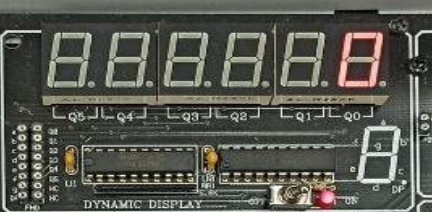
\includegraphics[width=0.5\textwidth]{images/result1}
	\caption{خروجی برنامه}
\end{figure}

\begin{figure}[h]
	\centering
	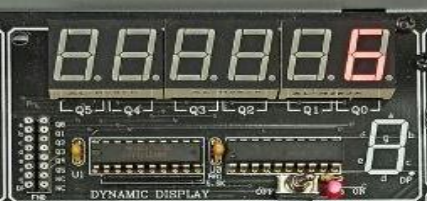
\includegraphics[width=0.5\textwidth]{images/result2}
	\caption{خروجی برنامه}
\end{figure}

\end{questions}
\end{document}